Die Übergangsfunktion stellt die Veränderung des Signals innerhalb des Systems als Funktion dar. Diese
kann durch Integrieren aus der Gewichtsfunktion (später dargestellt) gebildet werden. Dafür nutzt man wie
in den folgenden Abbildungen dargestellt den Laplace-Bereich, da nicht alle Funktionen einfach integriert
werden können.
\vspace*{0.5cm}
\begin{figure}[H]
    \begin{center}
        \fbox{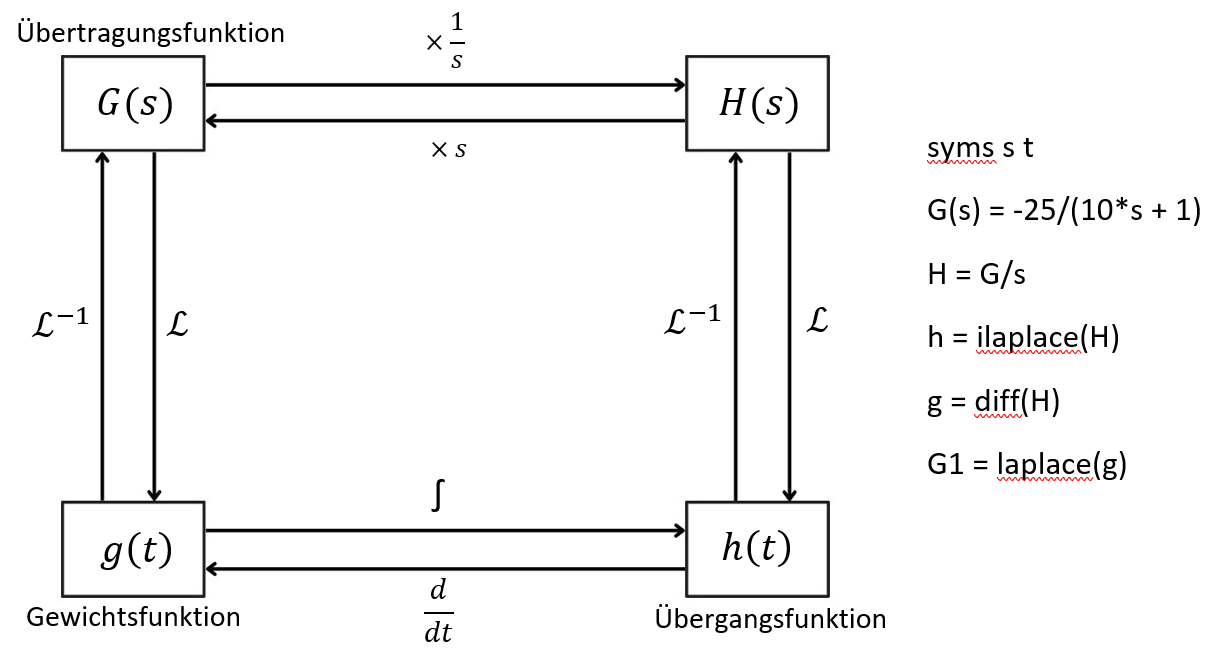
\includegraphics[width=13cm]{image/funktionen-fertig.png}}
    \end{center}
\end{figure}
\vspace*{0.5cm}
Der Vorteil der Laplace-Transformation ist, dass sich komplizierte Operationen der Analysis, wie bspw. Faltung, durch einfache Multiplikation im Laplace-Bereich äußern. Sofern man in der Klasse der linearen Zeitinvarianten Systeme (LTI) ist, sind die Laplace-Transformierten rationale Funktionen (Polynom/Polynom). Somit können Polynomdivision, Patialbruchzerlegung usw. angewendet werden.